

\subsection{Qubits and Quantum States}
\label{subsec:qubits}

\begin{definition}[Qubit]
A \emph{\gls{qubit}} is the fundamental unit of quantum information. It is represented as a normalised vector in a two-dimensional complex Hilbert space,
\[
\mathcal{H} = \mathbb{C}^2.
\]
\end{definition}

\begin{notation}[Computational Basis]
The standard (computational) basis states for a qubit are defined as
\[
|0\rangle = \begin{pmatrix} 1 \\ 0 \end{pmatrix}, \quad |1\rangle = \begin{pmatrix} 0 \\ 1 \end{pmatrix}.
\]
\end{notation}

\begin{definition}[General Qubit State]
A general state of a \gls{qubit} is given by
\[
|\psi\rangle = \alpha|0\rangle + \beta|1\rangle, \quad \text{with } |\alpha|^2 + |\beta|^2 = 1,
\]
where \(\alpha,\beta \in \mathbb{C}\) are the \emph{probability amplitudes}.
\end{definition}

\begin{remark}
Global phase factors—i.e. multiplying the state by an overall phase \(e^{i\gamma}\)—do not affect the physical properties of the qubit.
\end{remark}

\begin{example}[Bloch Sphere Representation]
  Any pure state of a \gls{qubit} can be written in the form
  \[
  |\psi\rangle = \cos\frac{\theta}{2}|0\rangle + e^{i\phi}\sin\frac{\theta}{2}|1\rangle,
  \]
  with \(\theta \in [0,\pi]\) and \(\phi \in [0,2\pi)\). Figure~\ref{fig:bloch_sphere} illustrates the \textbf{Bloch sphere} representation of a qubit \cite{nielsen2010quantum}.
\end{example}

\begin{figure}[h]
  \centering
  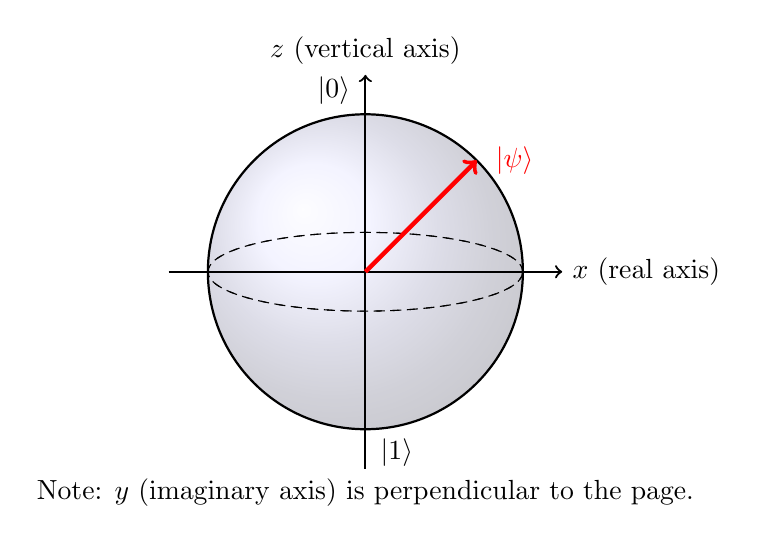
\begin{tikzpicture}[scale=1]
    % Draw sphere outline with shading
    \shade[ball color=blue!20, opacity=0.3] (0,0) circle (2cm);
    \draw[thick] (0,0) circle (2cm);
    
    % Draw equator as a dashed ellipse (horizontal cross-section)
    \draw[dashed] (0,0) ellipse (2cm and 0.5cm);
    
    % Draw meridian arcs (vertical cross-sections)
    \draw[dashed] (-2,0) arc (180:0:2cm and 0.5cm);
    \draw[dashed] (2,0) arc (0:-180:2cm and 0.5cm);
    
    % Axes: x and z
    \draw[->, thick] (-2.5,0) -- (2.5,0) node[right] {$x$ (real axis)};
    \draw[->, thick] (0,-2.5) -- (0,2.5) node[above] {$z$ (vertical axis)};
    
    % Mark north and south poles with horizontal shift
    \node[above, xshift=-0.4cm] at (0,2) {\(|0\rangle\)};
    \node[below, xshift=0.4cm] at (0,-2) {\(|1\rangle\)};
    
    % Bloch vector in the x-z plane
    \draw[->, red, ultra thick] (0,0) -- (1.414,1.414) node[right] {\(\;|\psi\rangle\)};
    
    % Note for y axis
    \node at (0,-2.8) {Note: \(y\) (imaginary axis) is perpendicular to the page.};
  \end{tikzpicture}
  \caption{Enhanced Bloch sphere representation of a \gls{qubit} with adjusted labels.}
  \label{fig:bloch_sphere}
  \end{figure}

\begin{observation}
  For multi-qubit systems, the overall state space is given by the tensor product of individual qubit spaces. For instance, a two-qubit system is described by
  \[
  |\psi\rangle = \sum_{i,j \in \{0,1\}} \alpha_{ij}\, |i\rangle \otimes |j\rangle, \quad \sum_{i,j} |\alpha_{ij}|^2 = 1.
  \]
  This exponential scaling of the state space underpins the potential of quantum parallelism \cite{nielsen2010quantum}.
\end{observation}


